\begin{figure}[h] 
\centering 
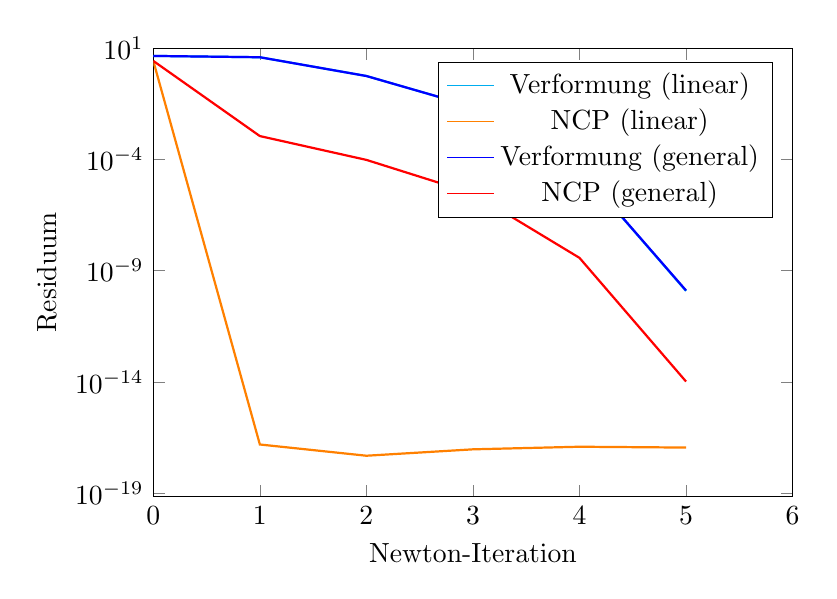
\begin{tikzpicture}[every plot/.append style={thick}] 
\begin{axis}[ 
label style={font=\normalsize}, 
xlabel={Newton-Iteration}, 
ylabel={Residuum}, 
xmin=0, xmax=6, 
ymode=log, 
ymin=0, ymax=10, 
width=0.8\textwidth, 
height=0.6\textwidth, 
legend pos=north east, 
legend style={cells={align=left}}, 
grid style=dashed, 
] 
\addplot[ 
color=cyan, 
] 
coordinates { 
(0, 4.48e+00)(1, 3.90e+00)(2, 5.62e-01)(3, 2.31e-02)(4, 4.00e-05)(5, 1.23e-10)}; 
\addlegendentry{Verformung (linear)} 
\addplot[ 
color=orange, 
] 
coordinates { 
(0, 2.67e+00)(1, 1.54e-17)(2, 4.81e-18)(3, 9.33e-18)(4, 1.22e-17)(5, 1.12e-17)}; 
\addlegendentry{NCP (linear)} 
\addplot[ 
color=blue, 
] 
coordinates { 
(0, 4.47e+00)(1, 3.91e+00)(2, 5.60e-01)(3, 2.33e-02)(4, 4.07e-05)(5, 1.29e-10)}; 
\addlegendentry{Verformung (general)} 
\addplot[ 
color=red, 
] 
coordinates { 
(0, 2.67e+00)(1, 1.12e-03)(2, 9.51e-05)(3, 2.94e-06)(4, 3.76e-09)(5, 1.04e-14)}; 
\addlegendentry{NCP (general)} 
\end{axis} 
\end{tikzpicture} 
\caption{Residuen des Stoffgesetzes 'St.Venant' mit Hinderniss 'Parabel' und 50 Freiheitsgraden für die Verschiebung.} 
\label{fiq:St.Venant_Parabel_level1} 
\end{figure} 
